\documentclass[a4paper,11pt,twoside]{report}
\usepackage[utf8]{inputenc}
\usepackage[top=2.5cm,bottom=2.5cm,outer=2.5cm,inner=2.0cm]{geometry}

\usepackage{amssymb}
\usepackage{amsmath}
\usepackage{booktabs}
\usepackage{hyperref}
\usepackage[noabbrev,capitalise]{cleveref}
\usepackage{colortbl}
\usepackage{color,soul}
\usepackage{xcolor}

\usepackage{enumitem}
% \setlist[enumerate,1]{label=\color{blue}(\arabic*)}
\setlist[enumerate,1]{label=(\arabic*)}

\usepackage{graphicx}
\usepackage{helvet}
\renewcommand{\familydefault}{\sfdefault}

\usepackage{hyperref}
\hypersetup{
	colorlinks = true,
	linkbordercolor = {white},
}

\usepackage{listings}

\usepackage{setspace}
\renewcommand{\baselinestretch}{1.3}

\usepackage{siunitx}
\usepackage{threeparttable}
\usepackage{multirow}

\renewcommand{\figurename}{SI Figure}
\renewcommand{\thefigure}{S\arabic{figure}}


\begin{document}

    \noindent {\large\textbf{Supplementary Information}}

    \begin{center}
        {\Large Accelerated Diffusion Weighted Magnetic Resonance Imaging at 7~T: Joint Reconstruction for Shift-Encoded Navigator-based Interleaved Echo Planar Imaging (JETS-NAViEPI)}
    \end{center}

    \begin{center}
        Zhengguo Tan, Patrick A. Liebig, Robin M. Heidemann, Frederik B. Laun, Florian Knoll
    \end{center}

    \vspace{2em}

    Here we aim to reproduce the results.
    Another subject with informed consent was recruited and
    measured by all protocols
    listed in Table 1 in the main manuscript.

    \newpage


    \begin{figure}[h]
        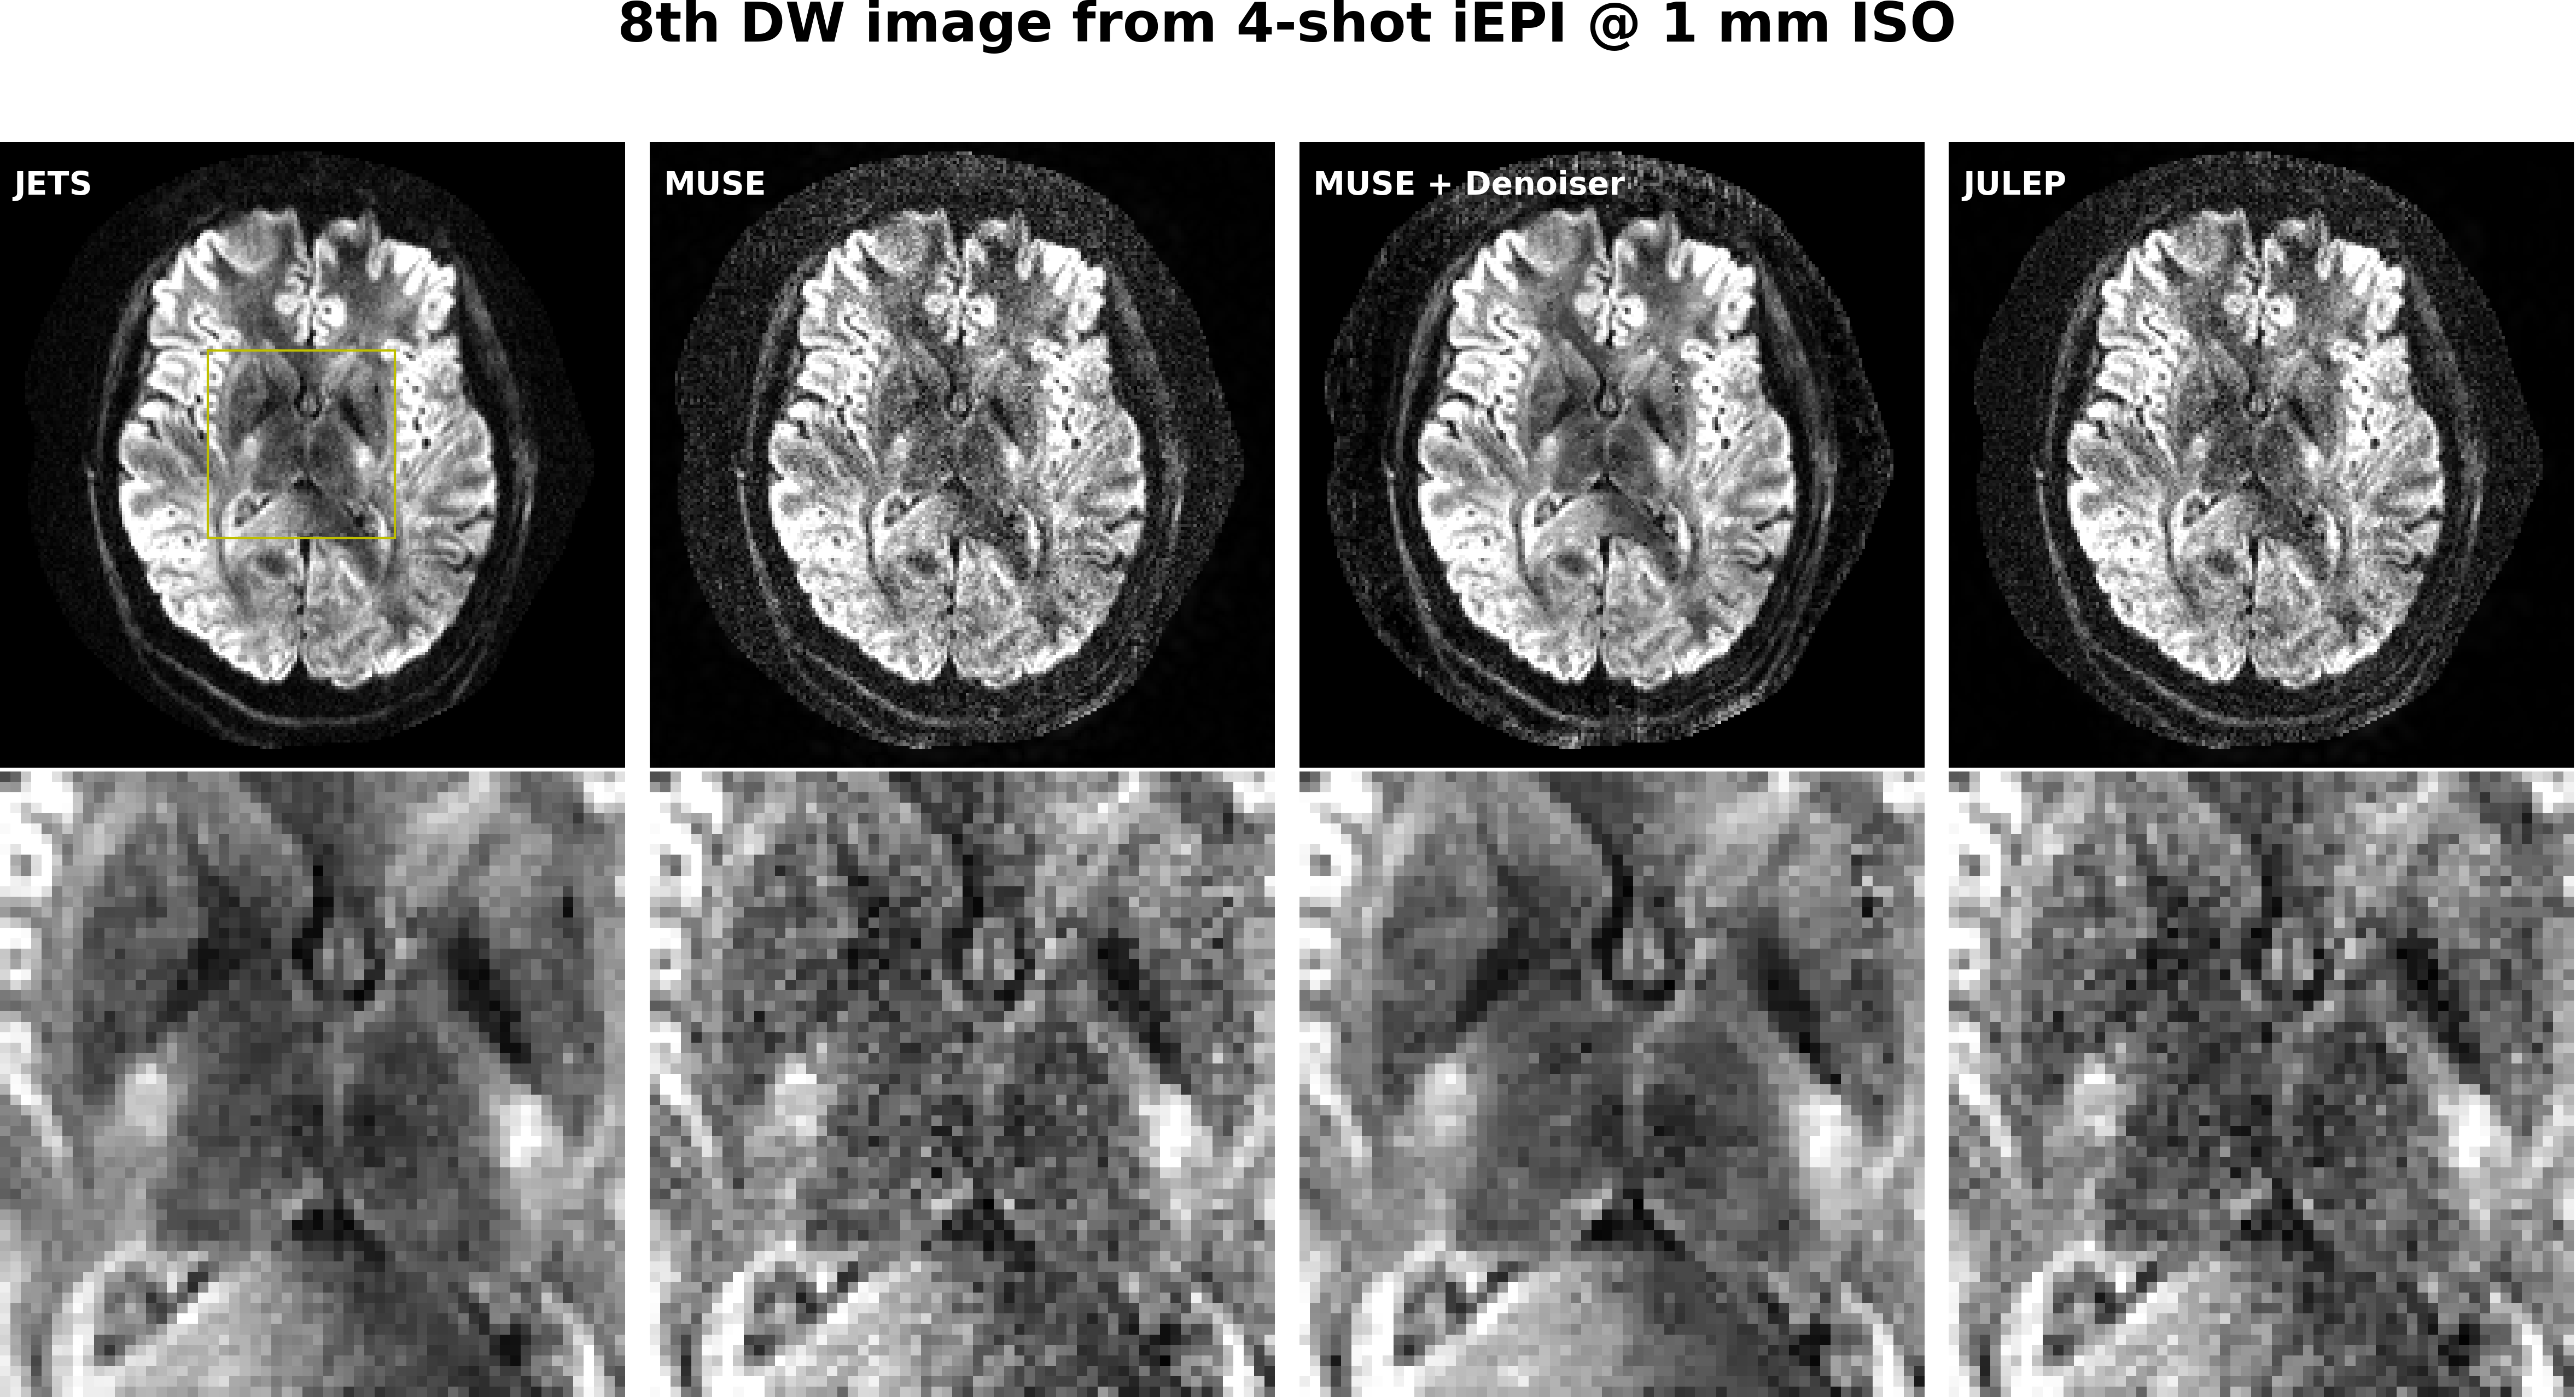
\includegraphics[width=\textwidth]{../figures/supp_fig1.png}
        \caption{Reproducing Protocol \#1.
        Reconstructed DW images
        (the 8th diffusion encoding)
        based on 4-shot iEPI acquisition with 1~mm isotropic resolution.
        Four reconstruction methods are compared (from left to right):
        JETS, MUSE, MUSE with denoiser, and JULEP.
        The 2nd row displays the magnified views of the yellow square.}
    \end{figure}

    \begin{figure}[h]
        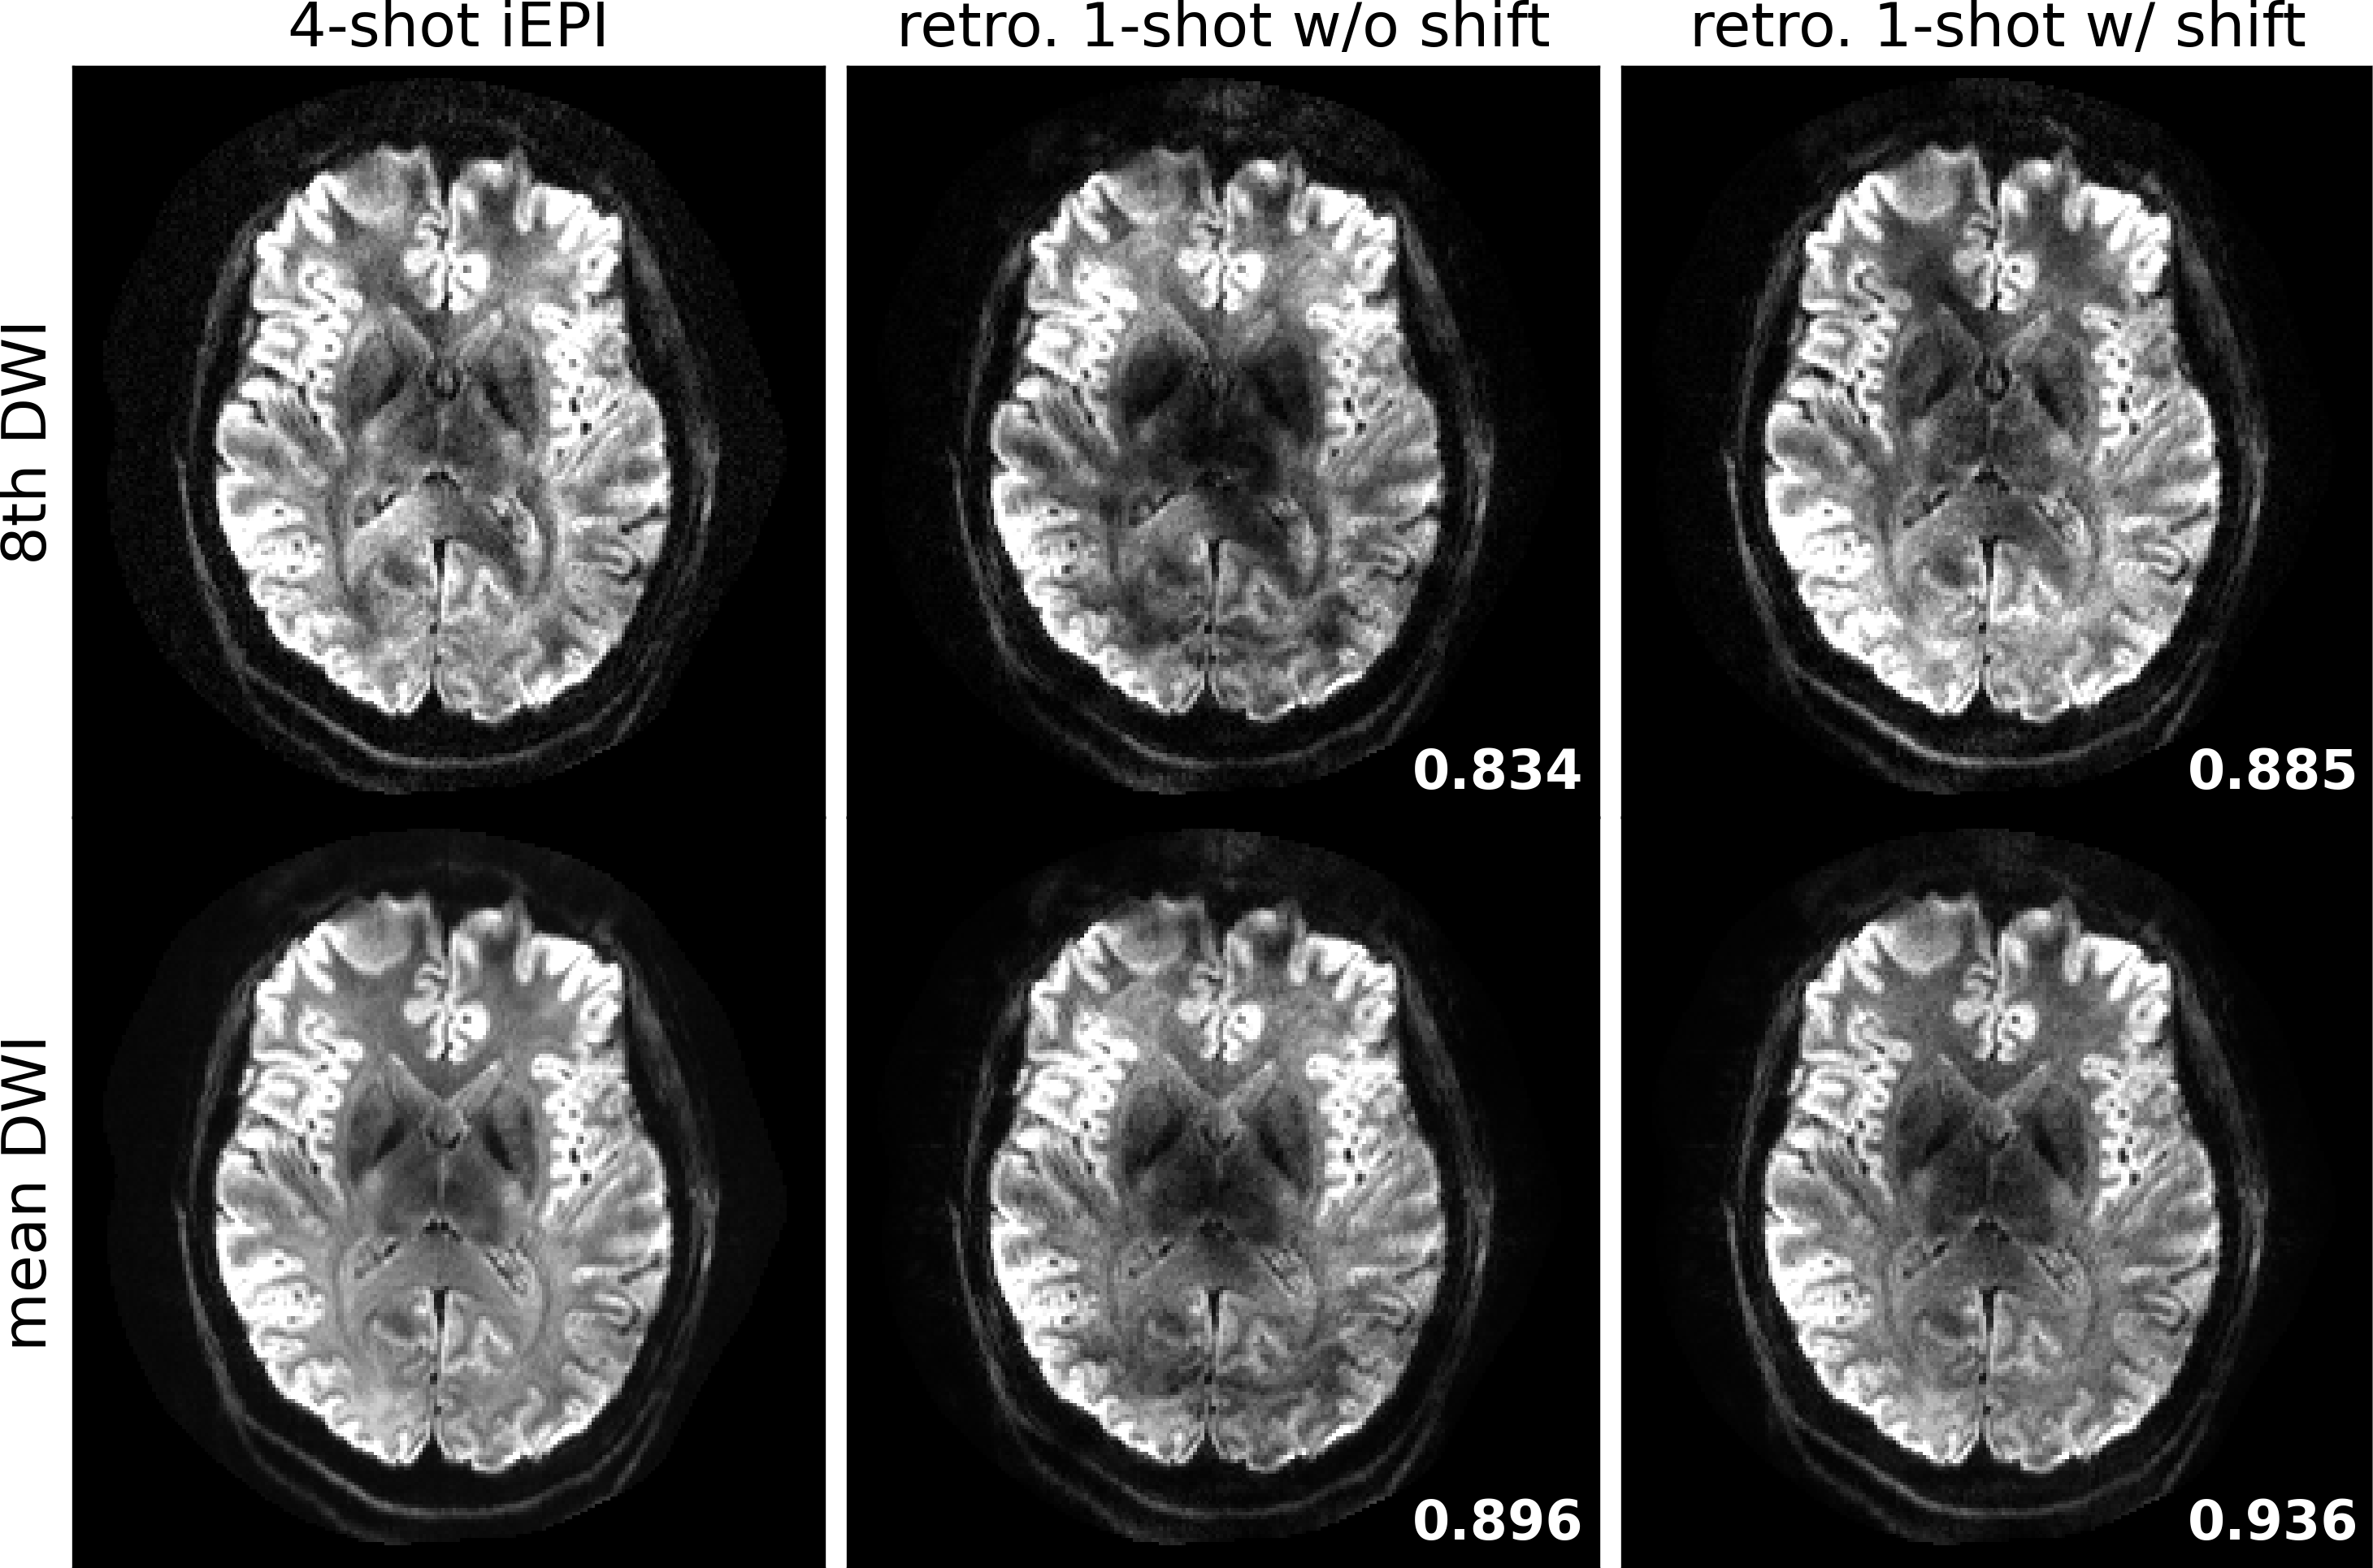
\includegraphics[width=\textwidth]{../figures/supp_fig2.png}
        \caption{Reproducing Protocol \#1.
        Quantitative validation of the proposed
        $k_y$-shift enoding sampling pattern
        based on 4-shot iEPI acquisition with 1~mm isotropic resolution.
        (Top) the 8th diffusion encoding and
        (bottom) mean DWI over 20 diffusion encodings.
        (1st column) JETS reconstruction of 4-shot iEPI acquisition
        is used as the ground truth.
        The 2nd and the 3rd column displays JETS reconstruction
        of retrospectively undersampled
        1-shot acquisition without and with $k_y$ shifting,
        respectively.}
    \end{figure}

    \begin{figure}[h]
        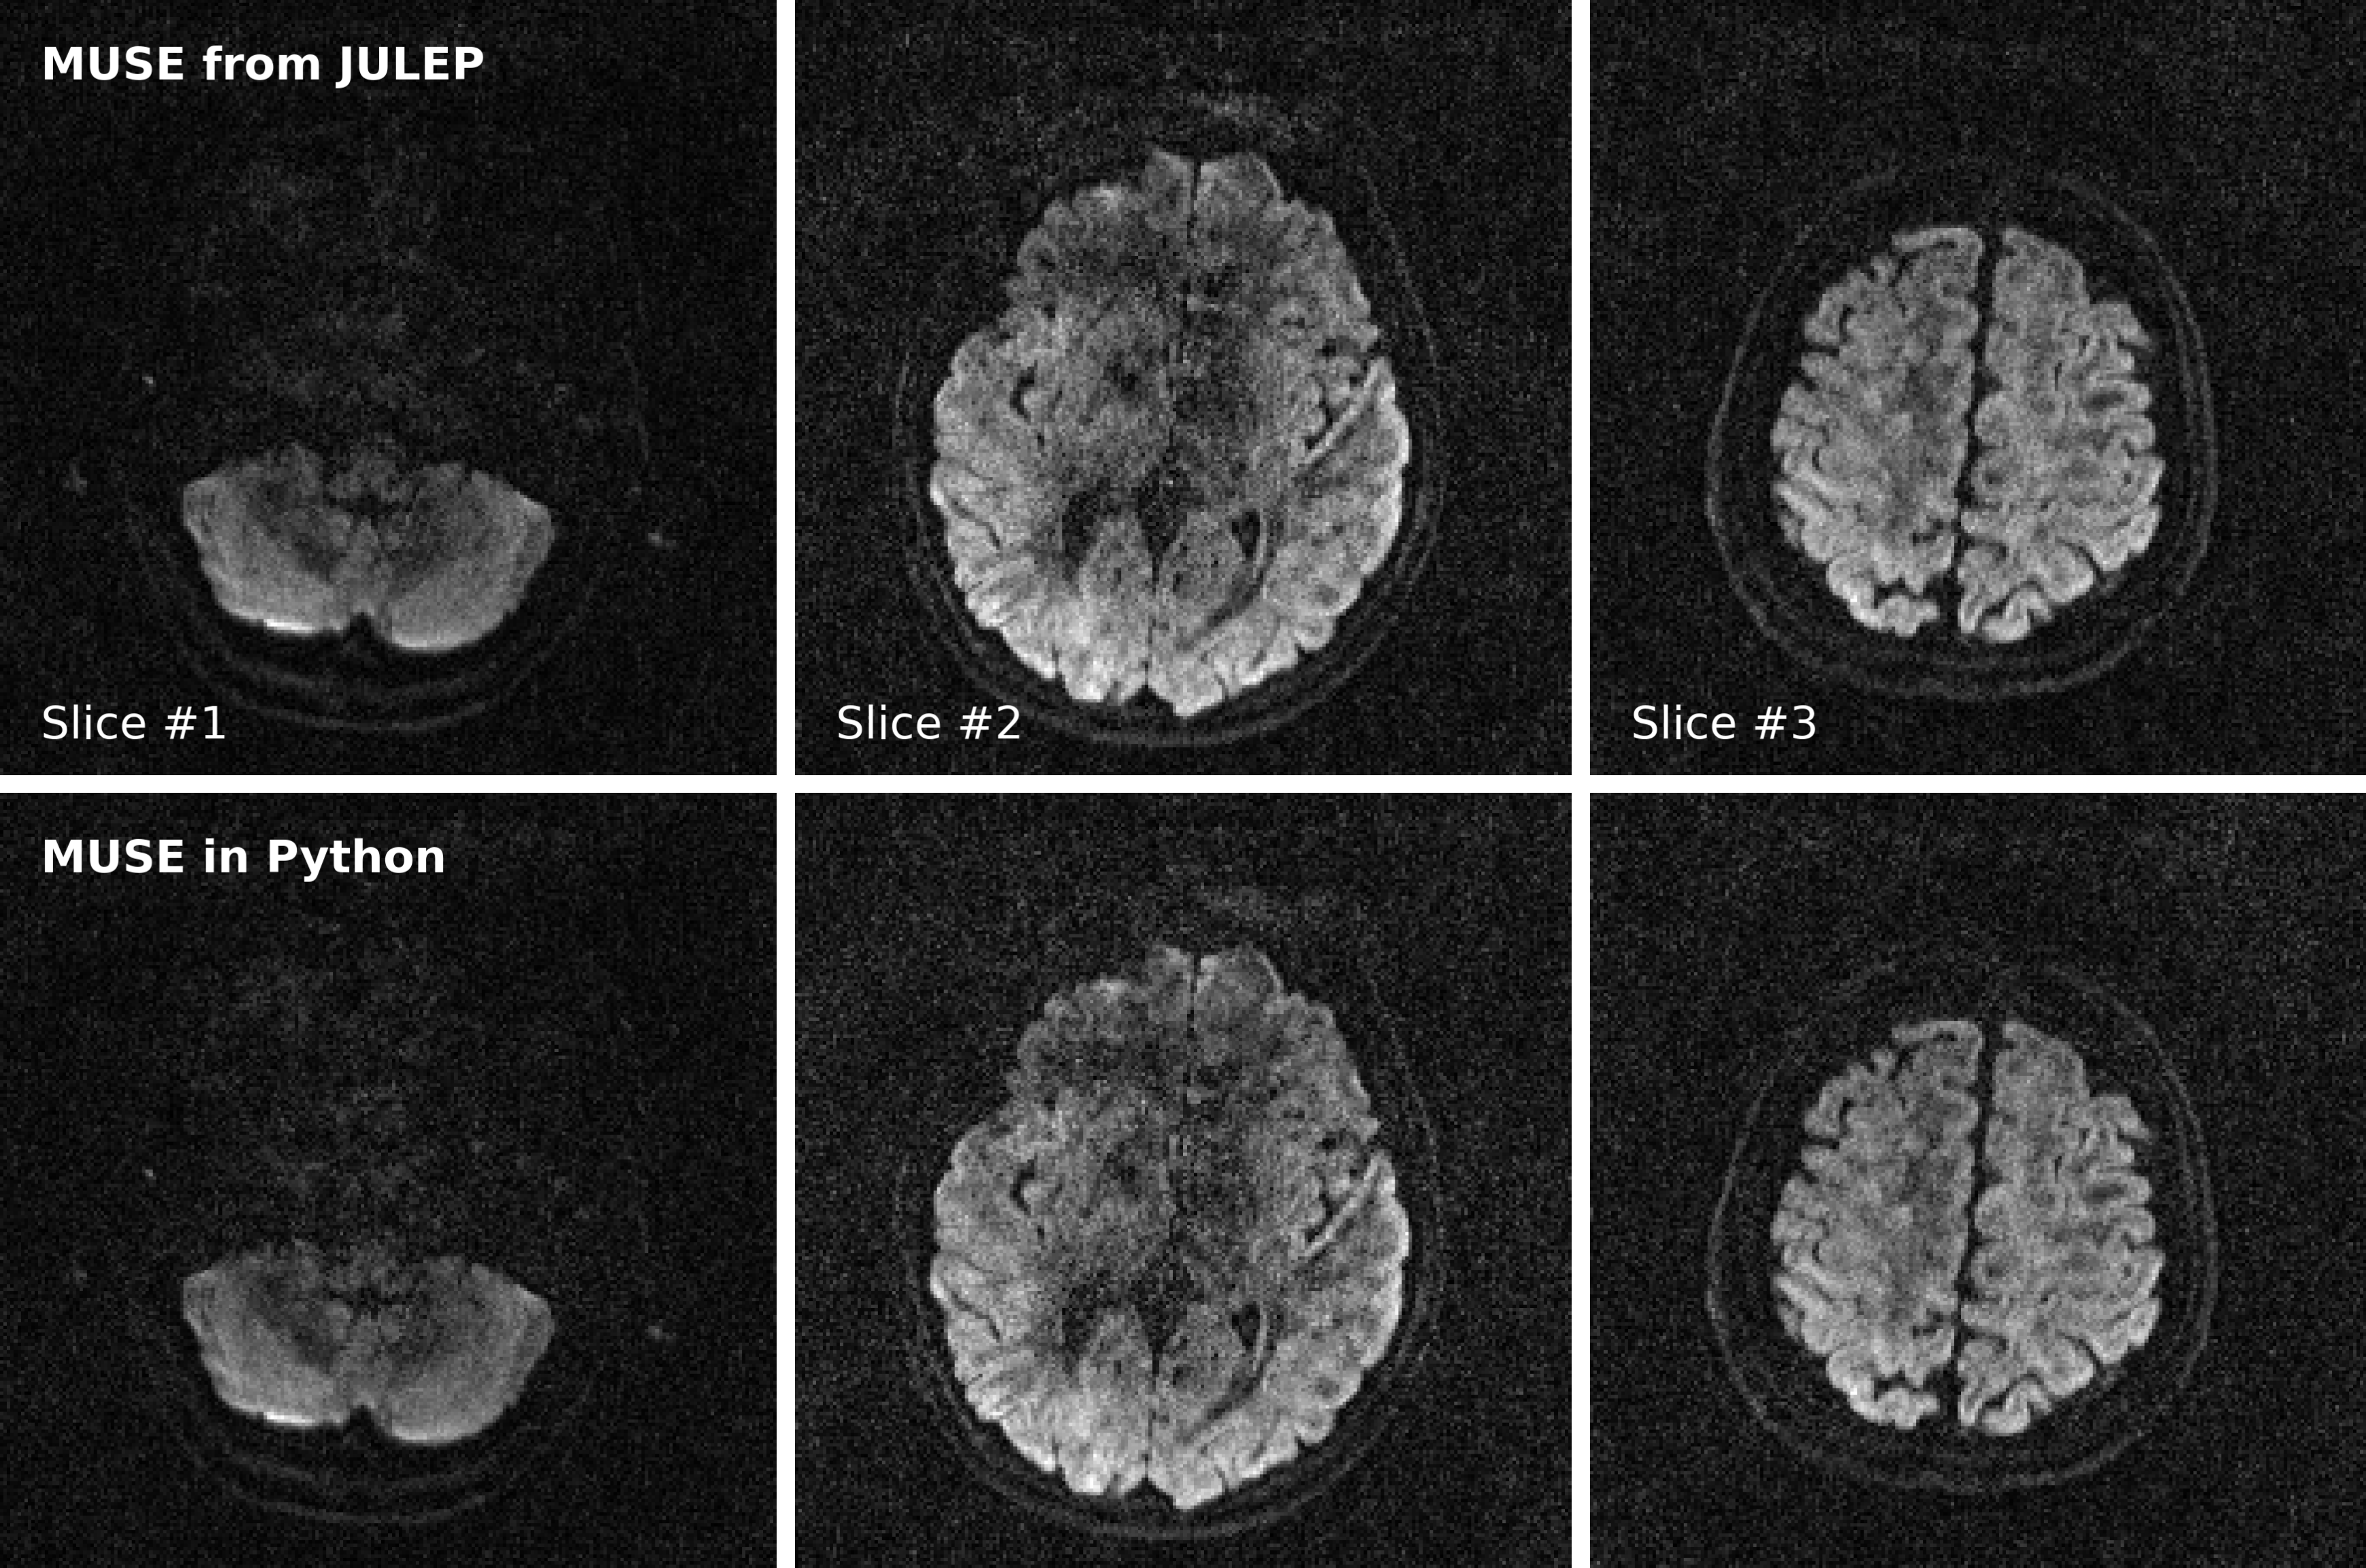
\includegraphics[width=\textwidth]{../figures/supp_fig4.png}
        \caption{Reproducing Protocol \#3.
        Reconstructed $b_0$ images from the 3-scan trace acquisition with
        the voxel size $0.5\times0.5\times2.0$~mm$^3$.}
    \end{figure}

    \begin{figure}[h]
        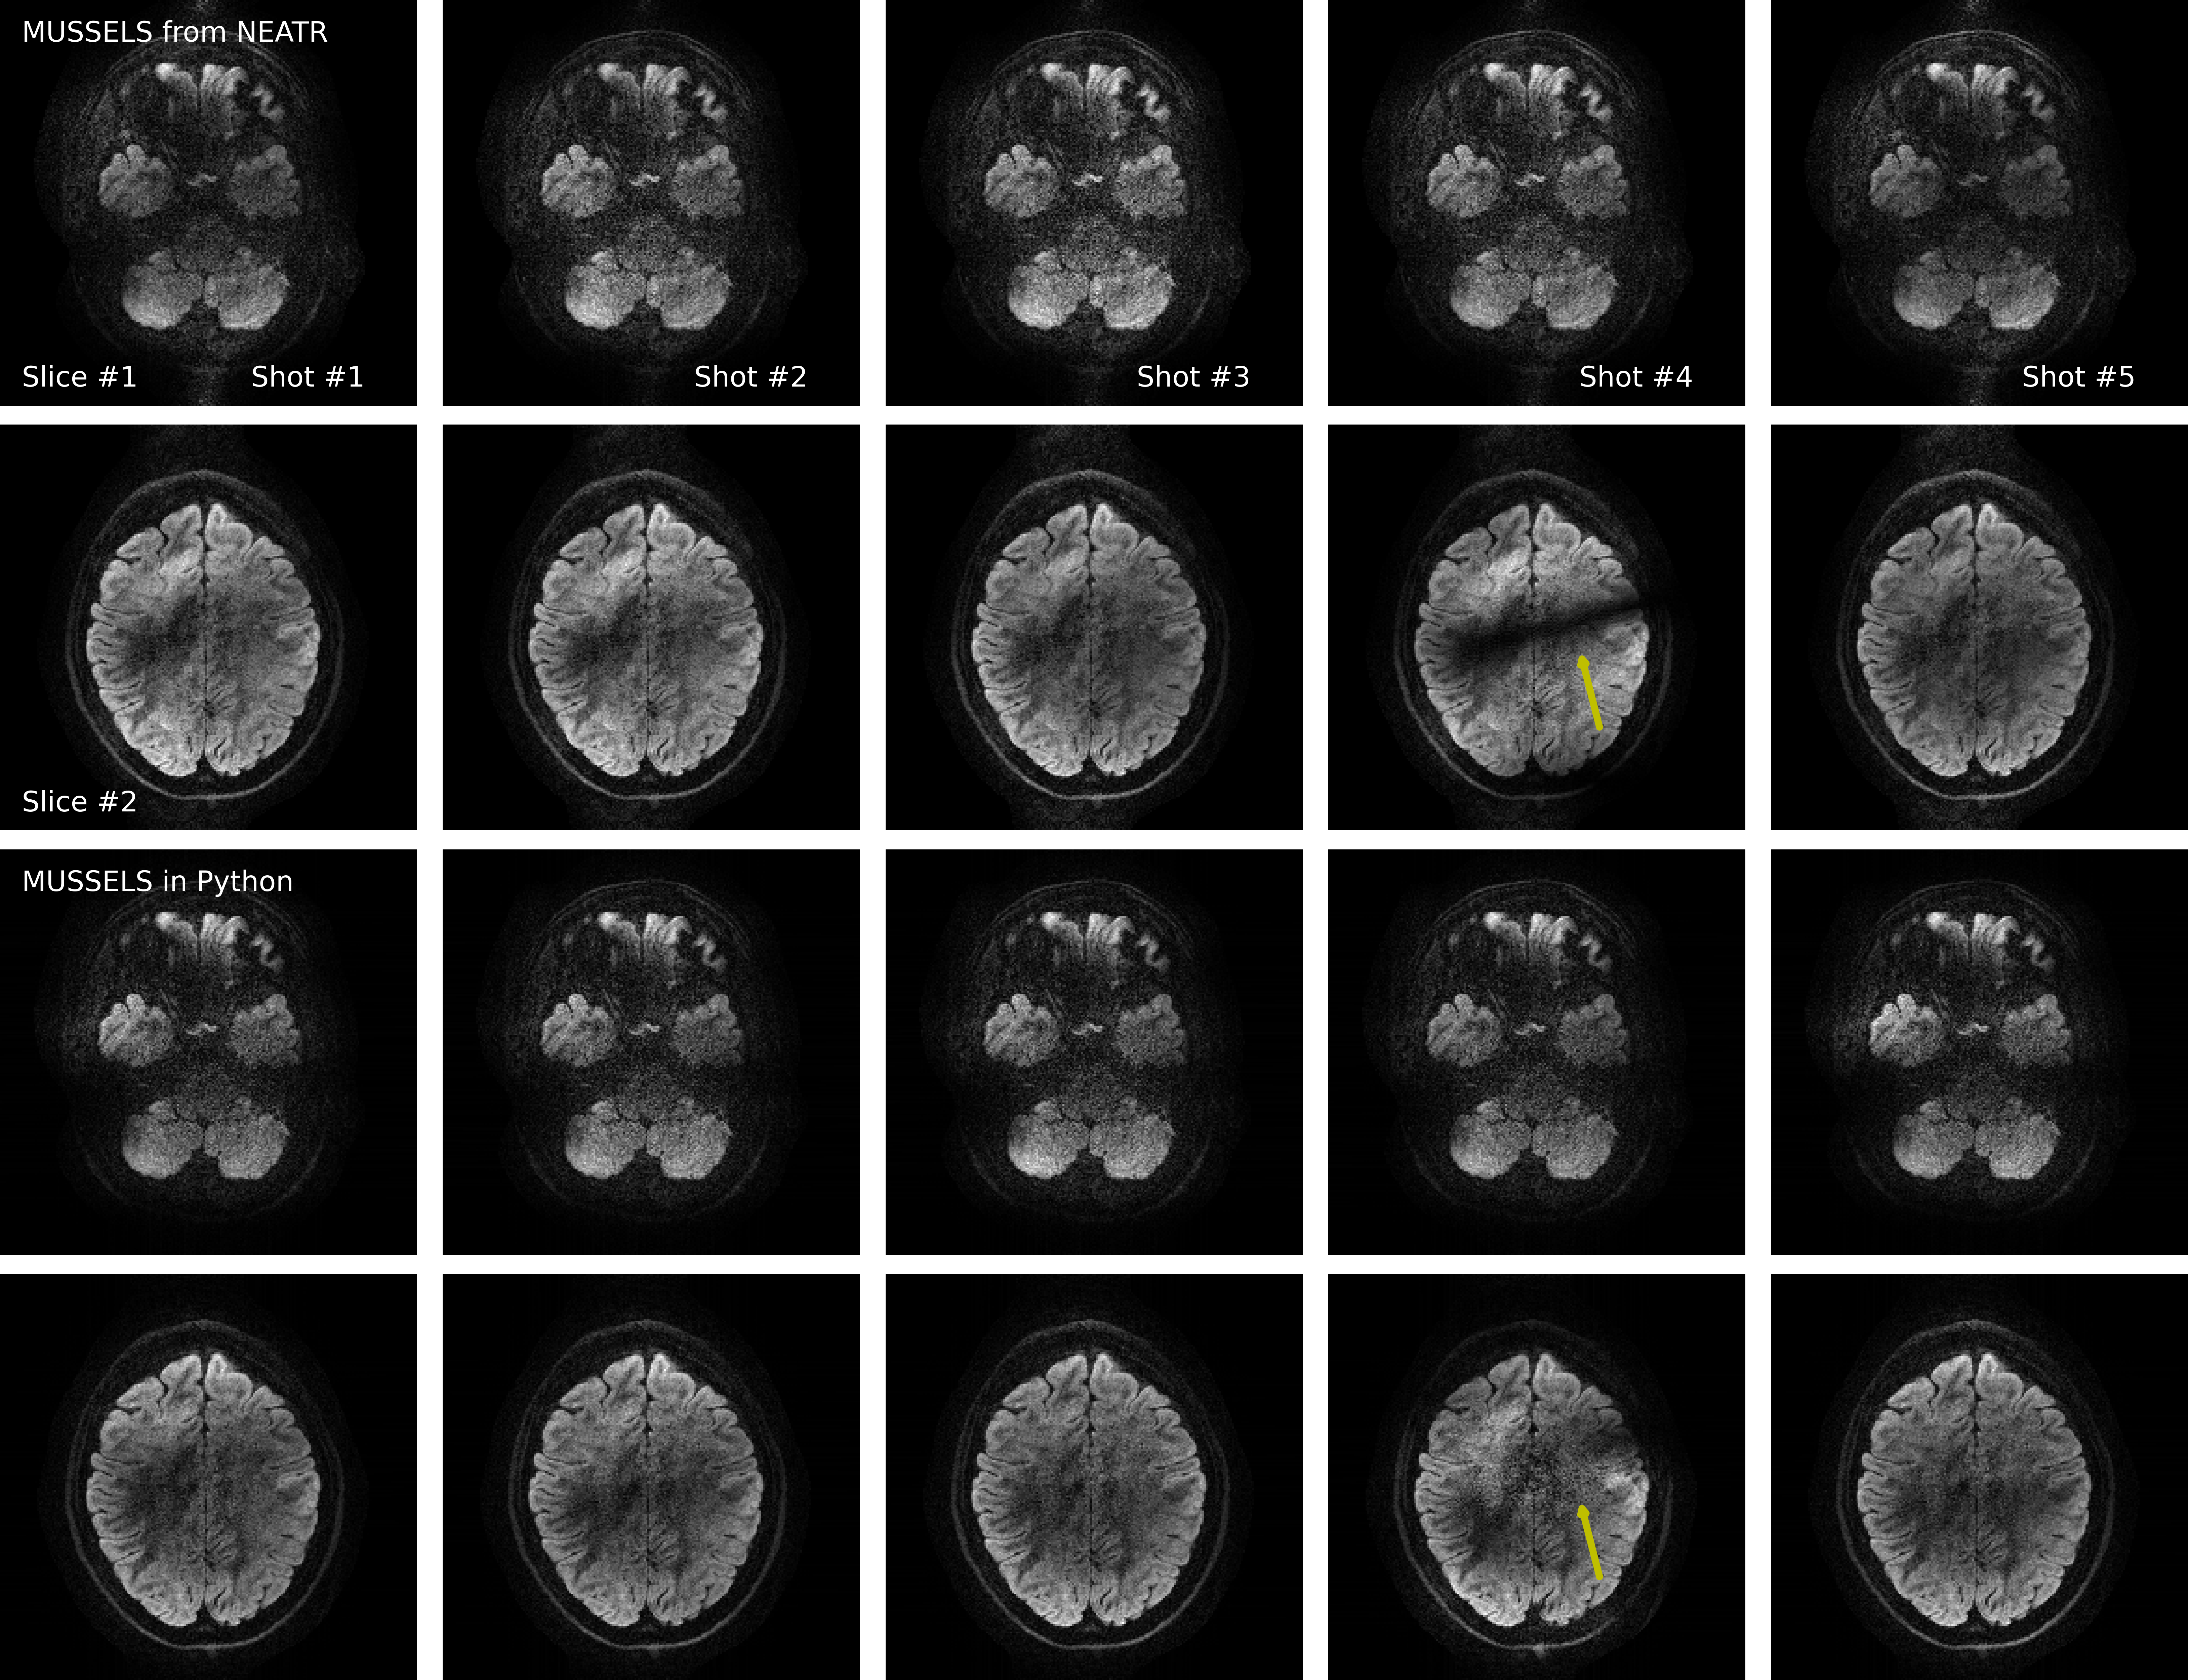
\includegraphics[width=\textwidth]{../figures/supp_fig5.png}
        \caption{Reproducing Protocol \#3.
        Reconstructed TRACE images from the 3-scan trace acquisition with
        the voxel size $0.5\times0.5\times2.0$~mm$^3$.}
    \end{figure}

    \begin{figure}[h]
        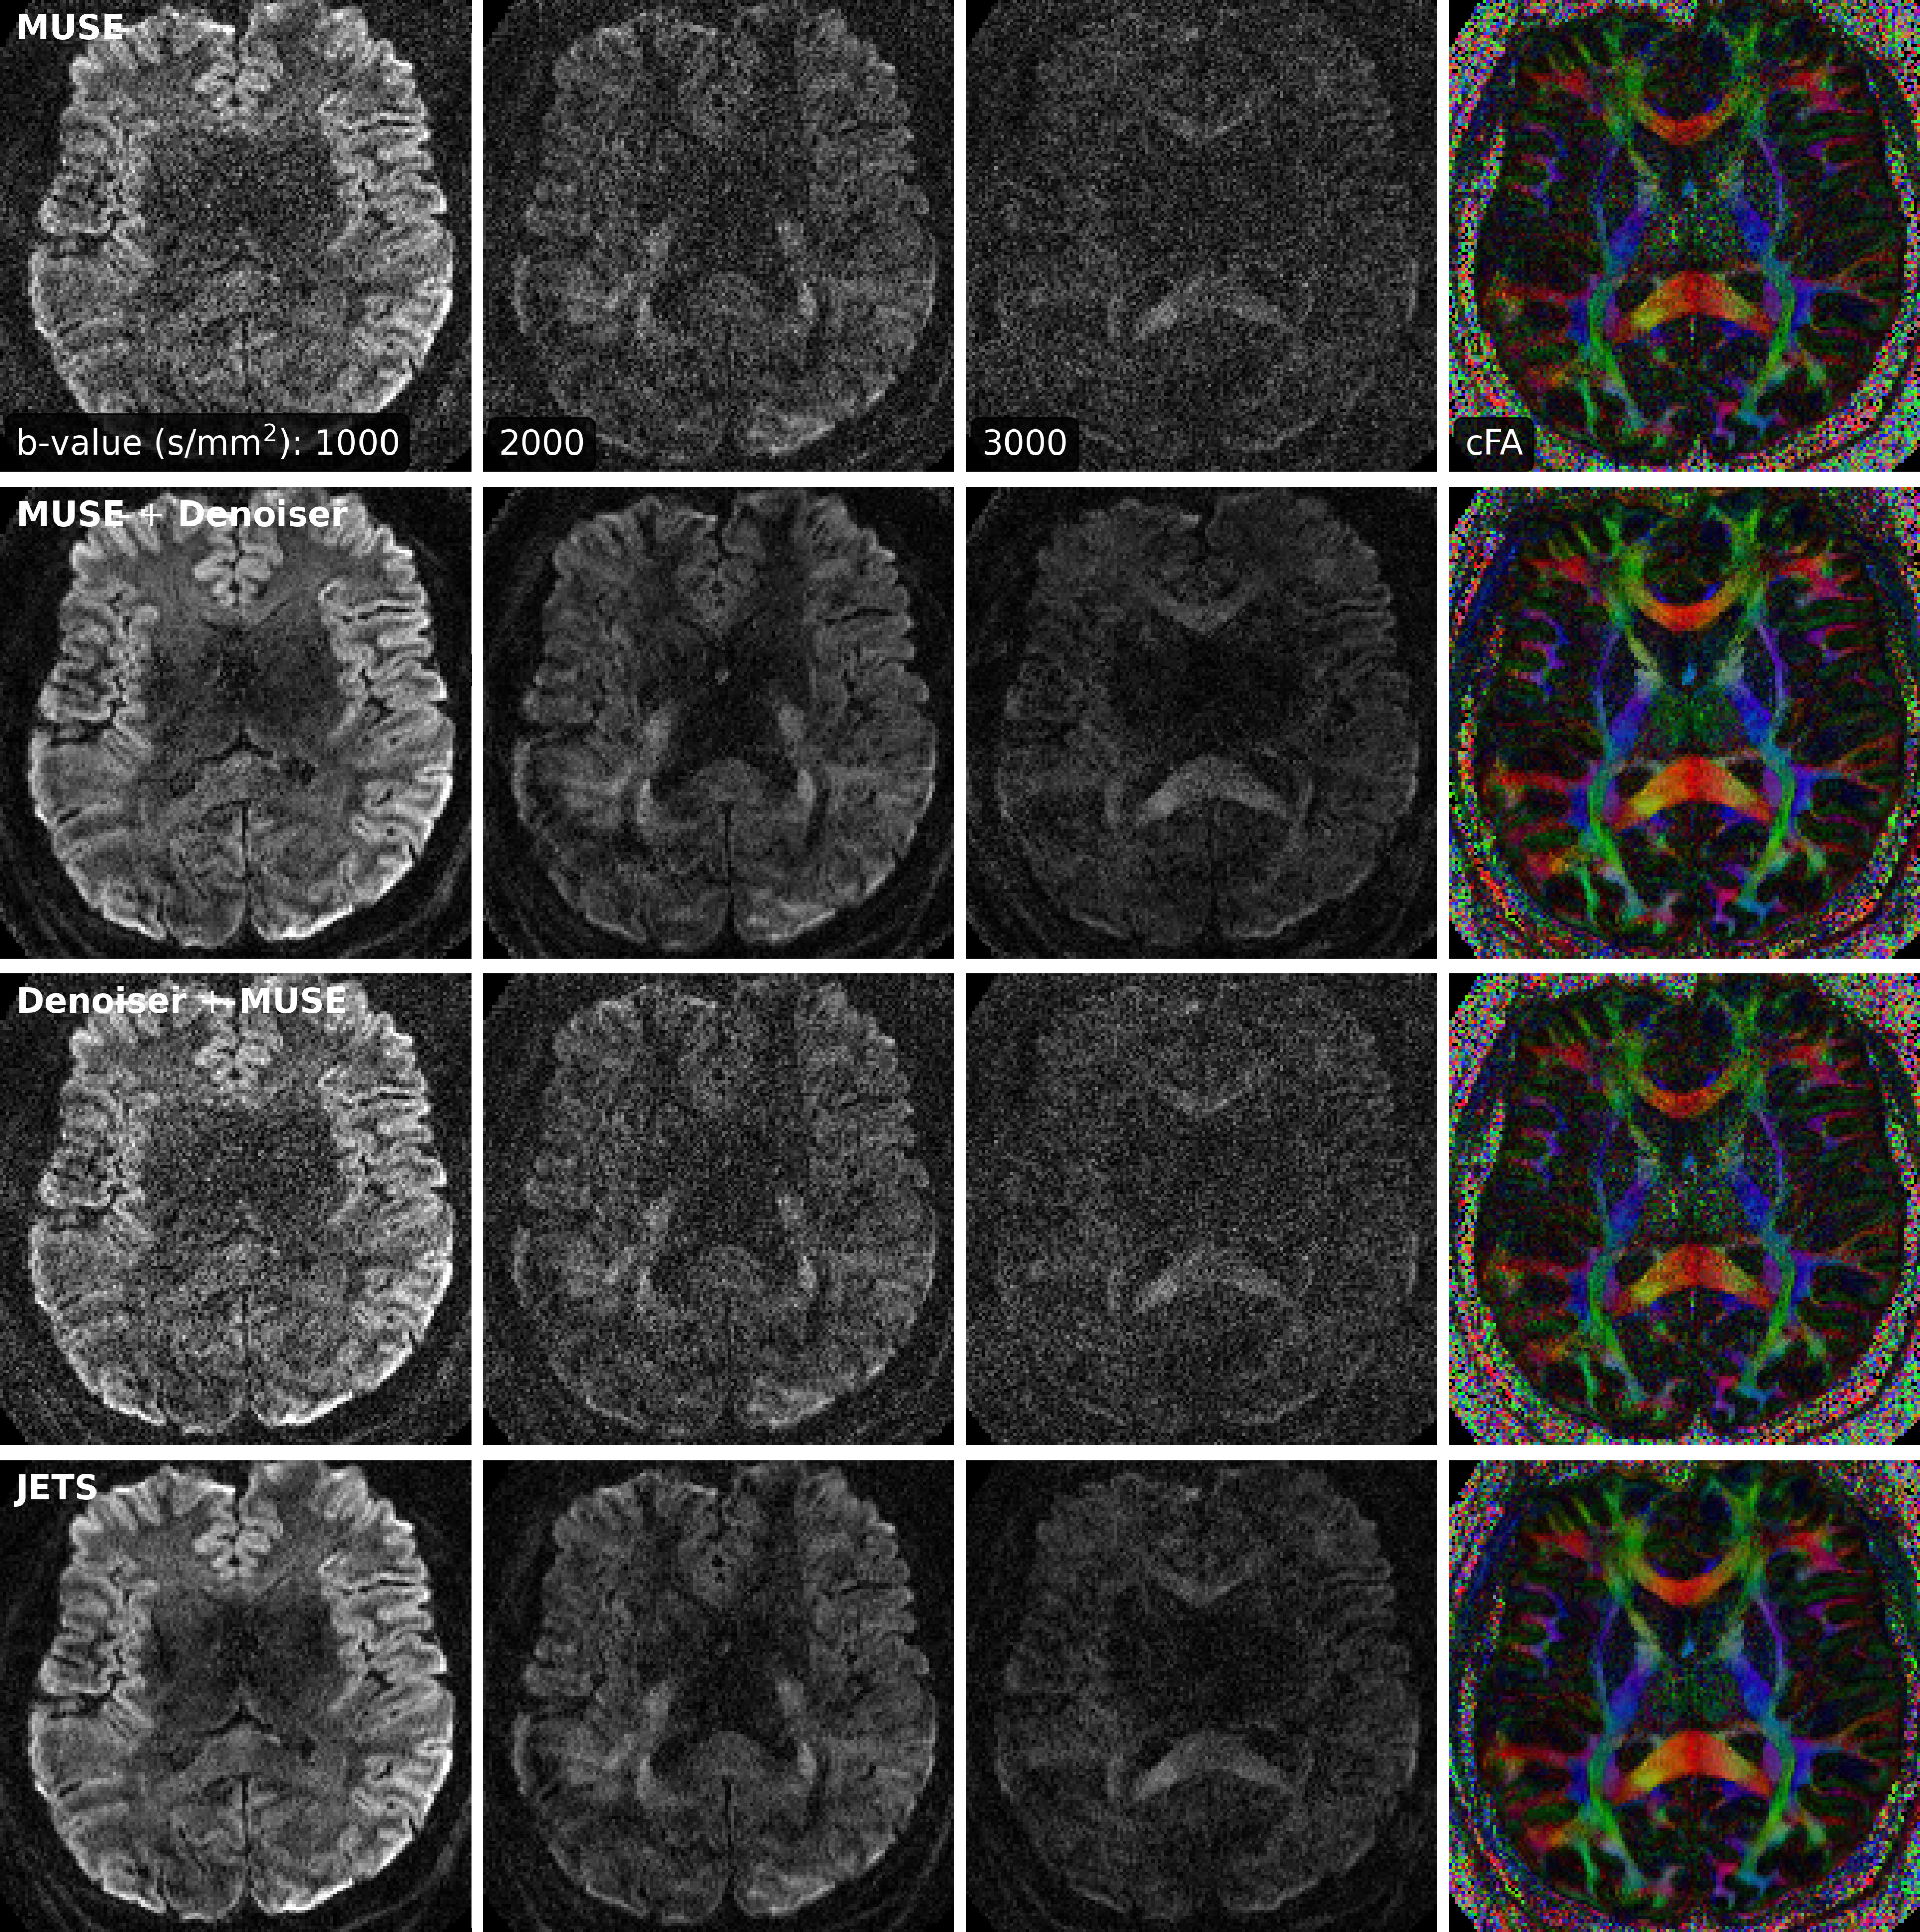
\includegraphics[width=\textwidth]{../figures/supp_fig6.png}
        \caption{Reproducing Protocol \#2.
        The FOV and bandwidth were adapted as
        \SI{200}{mm} and 1086~Hz/pixel, respectively.
        Comparison of three-shell DWIs and cFA maps
        reconstructed by (top to bottom)
        MUSE, MUSE with the local-PCA denoiser,
        MUSE with the local-PCA denoiser applied
        before the multi-shot combination,
        and the proposed JETS method, respectively.
        The local-PCA denoiser,
        when applied to shot images (3rd row),
        is less effective compared to
        its application to shot-combined images (2nd row).
        The reason is that shot images are reconstructed
        from the central $k$-space data,
        and thus have coarse resolution.}
        \label{SUPPFIG:6}
    \end{figure}

    \begin{figure}
        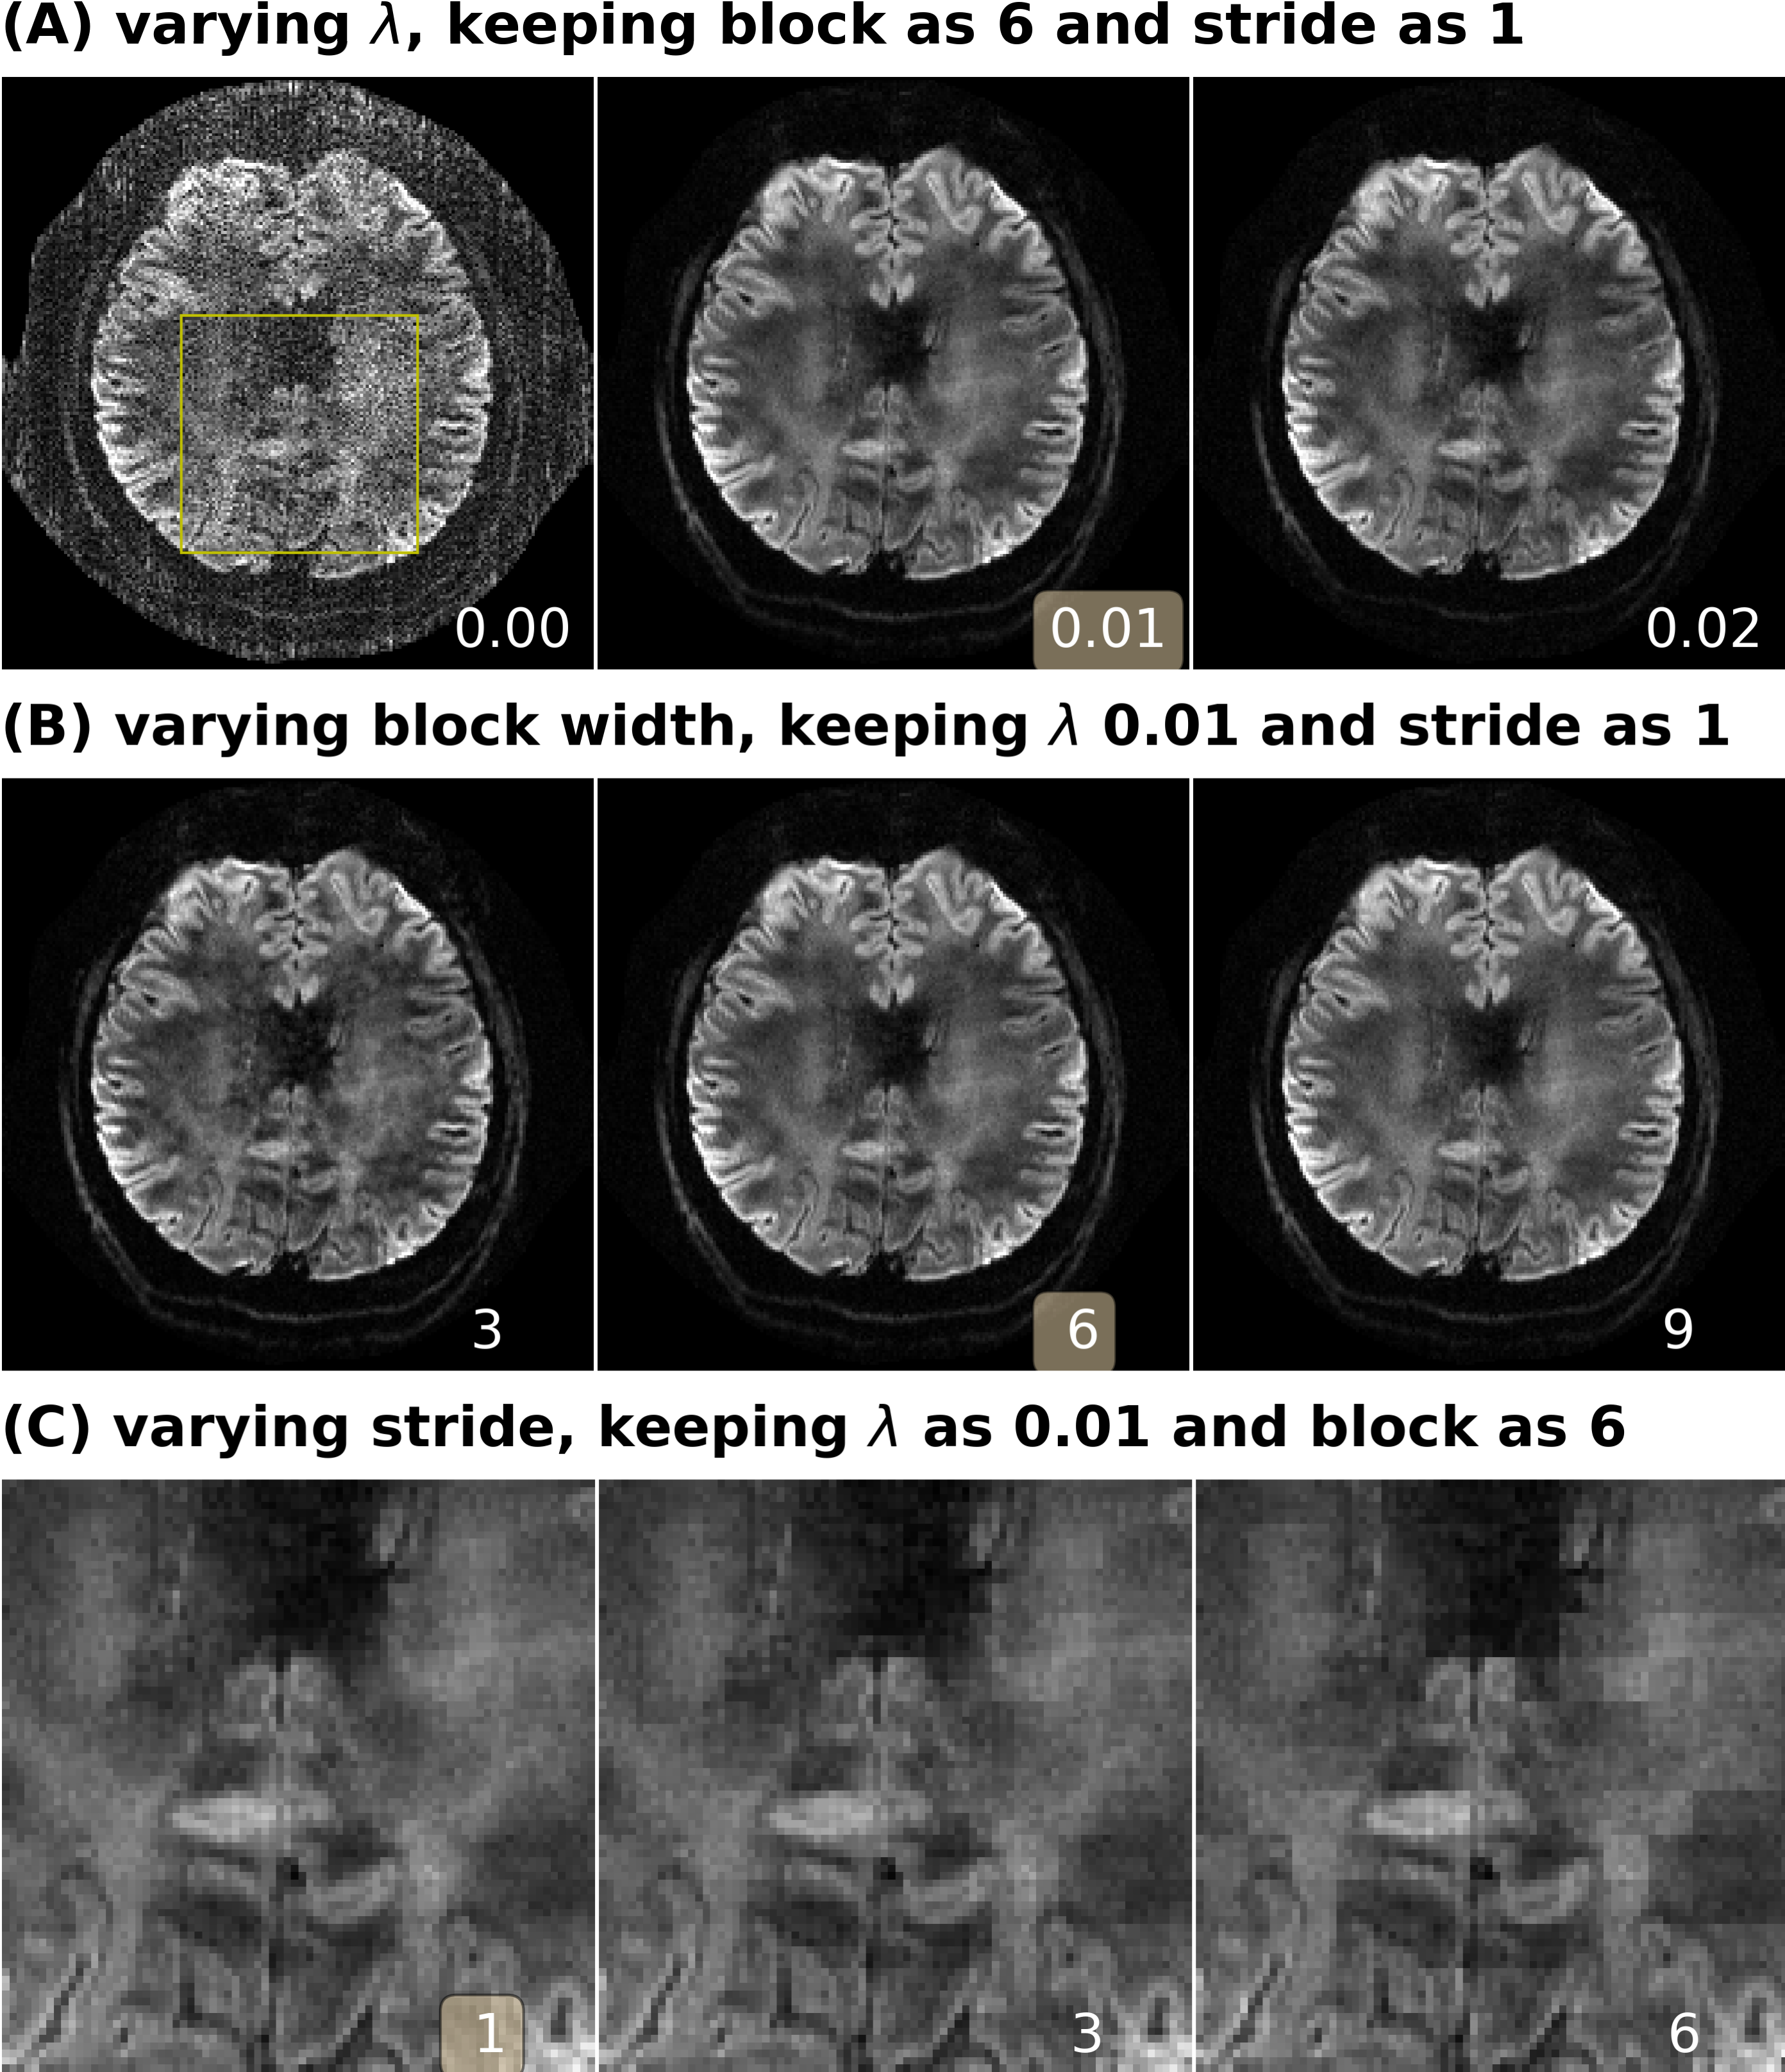
\includegraphics[width=\textwidth]{../figures/supp_fig7.png}
        \caption{Analysis of reconstruction parameters based on
        the 3-shell acquisition with 1~mm$^3$ isotropic resolution
        (Protocol \#2 in Table 1).
        Displayed are JETS reconstructed single-direction DW images.
        \textbf{(A)} Varying the regularization strength $\lambda$
        from $0$ to $0.01$ and $0.02$.
        \textbf{(B)} Varying the block width from $3$ to $6$ and $9$.
        The red arrow indicates increased noise
        with the large block width.
        \textbf{(C)} Varying the stride size from $1$ to
        $3$ (partially overlapping) and
        $6$ (non-overlapping).
        The red arrows indicate blocky artifacts.}
        \label{SUPPFIG:7}
    \end{figure}

\end{document}